\section{Hybrid approach}
\label{sec:hybrid-approach}
Lets look at all the candidate traversal strategies before explaining and
reasoning our decision tree.

\begin{table}[ht!]
\caption{Traversal strategies}
\label{tab:strategies}
\begin{tabular}{c|c}
Traversal stategy & Description \\\hline\hline
\textit{SEQ} & Sequential order \\\hline
\textit{INC} & Increasing order of node ids \\\hline
\textit{DEC} & Decreasing order of node ids \\\hline 
\textit{PO} & Post order \\\hline
\textit{RPO} & Reverse post order \\\hline 
\textit{WPO} & Worklist with post order \\\hline
\textit{WRPO} & Worklist with reverse post order \\\hline
\end{tabular}
\end{table}

\subsection{Candidate traversal strategies}
\label{sec:candidate-traversals}
\begin{itemize}
\item \textbf{\textit{Depth-first search (DFS)}} traverses a CFG by starting at
a arbitary node as root and explores as far as possible along each branch before
backtracking.\newline
\item \textbf{\textit{Post order traversal (POS)}} traverses the vertices in the
order that they were last visited by the algorithm. In CFGs that does not
contain loops, post order guarantees that a node will be visited only after
visiting its successors.
\item \textbf{\textit{Reverse post order traversal (RPS)}} is the reverse of a
postordering, i.e. a list of the vertices in the opposite order of their last
visit. In CFGs that does not contain loops, reverse post order guarantees that a
node will be visited only after visiting its predecessors.
\item \textbf{\textit{Worklist approach}} starts off with all nodes in a
worklist. Then a node is removed from the worklist and processed. If the state
changes, then its successors (for forward dataflow problems) or predecessors
(for backward dataflow problems) are added to the worklist.  Another node is
taken from the worklist if one exists and the process repeats until the list is
empty. Worklist approach visits nodes only on demand and removes redundant visit
of nodes. Worklist approach has two types.
\begin{itemize}
\item Worklist with post ordering of nodes : In this strategy,  worklist is
initialized with post ordering of nodes.
\item Worklist with reverse post ordering of nodes : In this strategy,  worklist
is initialized with reverse post ordering of nodes.
\end{itemize}
\item \textbf{\textit{Random traversal (RAN)}} traverses a CFG in random order
of its nodes.
\end{itemize}
There are two other non-standard traversal strategies mentioned below which were
created due to the property of our CFG nodes.
\begin{itemize}
\item \textbf{\textit{Traversing in the increasing order of node ids (IN-ID)}}
This traversal visits nodes in the increasing order of their node ids. We have a
property associates with the nodes in the CFG called node id. Node ids are
assigned while constructing the CFG of the program. Node ids are assigned in a
topological order. For sequential graph, traversing the graph in the increasing
order of node ids will give the flow of the program from entry point to exit
point.

\item \textbf{\textit{Traversing in the decreasing order of node ids (DC-ID)}}
This traversal visits nodes in the decreasing order of their node ids. For
sequential graph, traversing the graph in the decreasing order of node ids will
give the backward flow of the program.
\end{itemize}

% \begin{figure*}[ht!]
% \centering
% 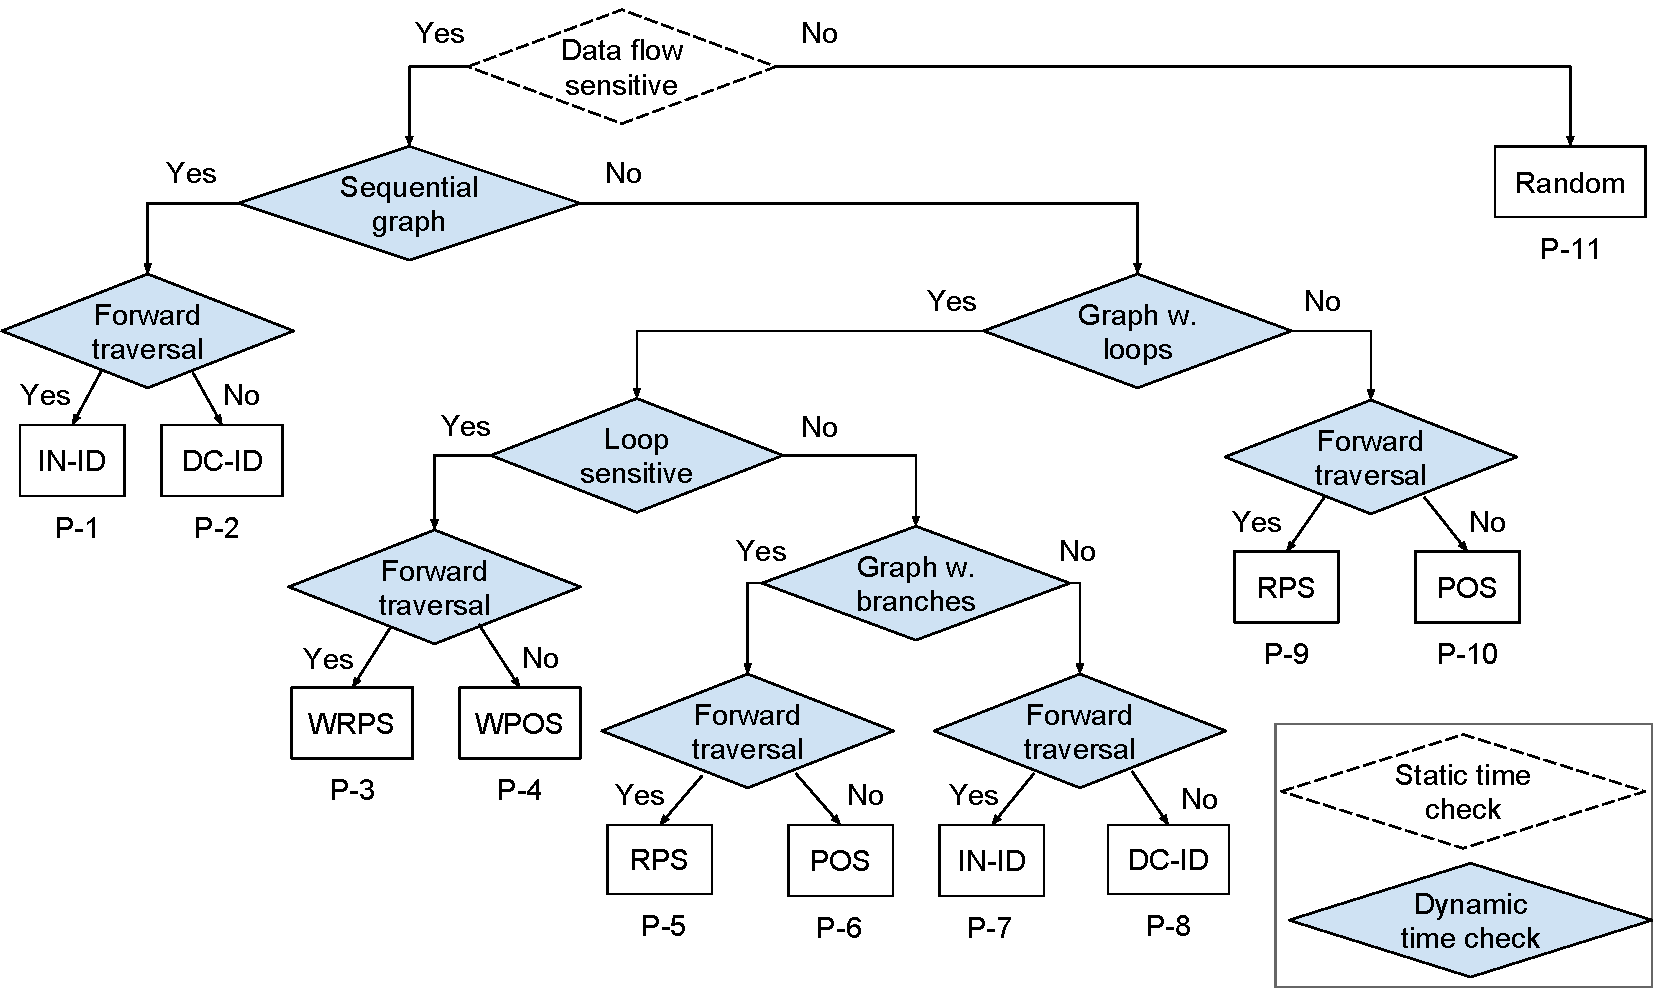
\includegraphics[width=\linewidth]{figures/tree.pdf}
%   \caption{Traversal strategy selection decision tree.}
% \label{fig:decision-tree}
% \end{figure*}
\begin{figure}[ht!]
\centering
\includegraphics[width=\linewidth]{figures/decision.png}
\caption{Traversal strategy selection decision diagram. $P_0$ to $P_{11}$ are
markings for paths.}
\label{fig:decision-diagram}
\end{figure}

Let us reason the decisions taken by the decision tree and the optimizations
performed on it.
\subsection{Reasoning of the Decision tree}
\label{sec:Decision tree explained}
First, we check if the traversal is data flow sensitive or not. We distinguish
the traversal based on this property because traversal without data flow
completes in a single traversal of the CFG, while data flow sensitive traversal
traverses the CFG multiple time till all the nodes reach fixpoint ie the ouput
of all the nodes stabilizes. Hence the decision making process differs based on
the data flow  property. Lets look at the decision tree if the traversal is data
flow sensitive.\newline
\subsubsection{Decision tree for data flow sensitive traversal}
For data flow sensitive traversal, we look at the type of the control flow in
the CFG. This property is important now because the type of control flow
determines the number of traversal needed for data flow sensitive traversal.
\paragraph{Sequential CFG} \label{sec:decision-ds-seq}
If the graph is sequential, it means the CFG has no branches or loops. When we
know this property of graph, we can see that solving the data flow equations is
straightforward. Each node has only one predecessor/successor and hence if the
nodes are ordered in such a way that it is processed only after it's predecessor
(forward traversal) or it's successor (backward traversal), then the sequential
CFG will attain fix point in single traversal.
In order to get this ordering for sequential graph, we just have to traverse the
graph in the increasing of order of the CFG node ids (IN-ID) for forward
traversal and decreasing order of node ids (dc-id) for backward traversal. This
is because node ids are assigned in topological order as they are created and
for sequential graphs with no branches or loops, traversing the graph in the
increasing order of node ids will ensure that we traverse the node's predecessor
before the node itself. Traversing the graph in the decreasing order of node ids
will ensure that we traverse the node's successors before the node itself. Hence
hybrid traversal picks IN-ID for forward traversal and DC-ID for backward
traversal approach for sequential CFG. P-1 and P-2 in figure
\ref{fig:decision-tree} are the paths that lead to these decisions.\par
\textit{Optimization on the chosen traversal} : From the knowledge that the
graph is sequential and the traversal is data flow sensitive, hybrid approach
knows that IN-ID for forward traversal and DC-ID for backward traversal, will
complete the data flow sensitive traversal in first iteration of the CFG and we
do not have to check fixpoint in the first iteration to confirm it. Hence hybrid
approach removes fixpoint checking operation.\par

Approaches like DFS, POS, RPS, RAN will take two iteration to realize that we
have reached fix point in the first traversal, which is an overhead and an
unwanted traversal. WPOS and WRPS will visit only as much nodes as needed but it
will add an overhead of creating and maintaining the worklist. Also approaches
like DFS, POS, RPS involves accessing edge informations to determine the next
node to visit while IN-ID and DC-ID already has the nodes in order and just
visits them.\par

If the CFG is not sequential, then we check if the CFG has loops.
\paragraph{CFG with branches and no loop} \label{sec:decision-ds-br}
If the CFG does not have loop, then it is a CFG with branches and no loops. When
we know this property of graph, we can see that this CFG will stabilize in
single traversal if all predecessors of the node have been processed before the
node itself(for forward traversal) or if all the successors of the node have
been processed before the node itself(for backward traversal). RPS guarantees
such ordering for forward traversal and POS guarantees such ordering for
backward traversal. Hence hybrid picks RPS for forward traversal and POS for
backward traversal. P-9 and P-10 in figure \ref{fig:decision-tree} are the paths
that lead to these decisions.\par \textit{Optimization on the chosen traversal}
: From the knowledge that the graph has only branches and the traversal is data
flow sensitive, hybrid approach knows that RPS for forward traversal and POS for
backward traversal, will complete the data flow sensitive traversal in first
iteration of the CFG and will complete the data flow sensitive traversal in
first iteration of the CFG and we do not have to check fixpoint in the first
iteration to confirm it. Hence hybrid approach removes fixpoint checking
operation.\par Approaches like DFS, RAN, IN-ID, DC-ID will take multiple
iteration to reach fix point. WPOS and WRPS has an overhead of creating and
maintaining the worklist.

\paragraph{CFG with loops}
If the CFG has loops, it may or may not have branches other than the loop. We
next determine if the traversal is loop sensitive or not.\par \textbf{Loop
insensitive} : If the traversal is insensitive to loop, then we can just ignore
the loops present in the CFG and make decision based on the structure of the
rest of the CFG. If the CFG have branches other than the loop, then hybrid picks
RPS for forward traversal and POS for backward traversal based on the
explanation in Section \ref{sec:decision-ds-br}. P-5 and P-6 in figure
\ref{fig:decision-tree} are the paths that lead to these decisions. If the CFG
does not have branches other than the loop, then hybrid picks IN-ID for forward
traversal and DC-ID for backward traversal based on the explanation in Section
\ref{sec:decision-ds-seq}. P-7 and P-8 in figure \ref{fig:decision-tree} are the
paths that lead to these decisions.\par \textbf{Loop sensitive} : If the
traversal is loop sensitive and the CFG has loops, then no ordering of nodes can
guarantee fix point convergence in single traversal. Worklist approach is the
near best here as it visits node only on demand. Hybrid approach chooses WRPS
for forward traversal and WPOS for backward traversal. P-3 and P-4 in figure
\ref{fig:decision-tree} are the paths that lead to these decisions.\par
--------------discussion needed on why worklist is near best and not the
best-----------------\par Now let us look at the decision tree if the traversal
is data flow insensitive.
\subsubsection{Decision tree for data flow insensitive traversal}
% We check if the traversal is sensitive to the traversal strategy used.
% Traversal sensitivity means the output of the traversal changes from one
% traversal strategy to another. If the traversal is sensitive to the traversal
% strategy, then hybrid cannot pick the best strategy as we may compromise on
% the soundess of the result. We did not check this property when the traversal
% is data flow sensitive. This is because, even if data flow traversal is
% traversal sensitive, we will run the traversal till the fixpoint is reached
% and hence we will end up with the correct result.\par
If the traversal is data flow insensitive, then hybrid approach picks random
traversal. This is because since there is no data flow in the traversal, the
traversal is local to the node and is not dependent on the output of other nodes
and hence the nodes could be visited in any order.\par Other approaches like
DFS, POS, RPS involves accessing edge informations to determine the next node to
visit while WPOS and WRPS has an overhead of creating the worklist. IN-ID and
DC-ID has an unwanted contraint of accessing the nodes in order, which is an
overhead.\par Let us look at the algorithms that computes the required static
and dynamic properties.
\subsection{Computation of static properties}
\label{sec:static}
\begin{algorithm}[ht!]
\caption{Algorithm to detect data-flow sensitivity}
\label{algo:flow-sensitive}
\KwIn{\lstinline|t := traversal(n : Node) : T \{ tbody \}|}
\KwOut{\textit{true/false}}
$A$ $\leftarrow$ \textit{getAliases}(\lstinline|tbody|, \lstinline|n|)\;
\ForEach{ \lstinline|stmt| $\in$ \lstinline|tbody|}{
	\If{$stmt$ $=$ \lstinline|output(n', t')|}{
		\If{\lstinline|t'| $==$ \lstinline|t| and \lstinline|n'| $\notin$ $A$ }{
			return \textit{true}\;
		}
	}
	
}
return \textit{false}\;
\end{algorithm}

%\begin{wrapfigure}{R}{.5\textwidth}
\begin{algorithm}
\caption{Algorithm to detect loop sensitivity}
\label{algo:loop-sensitive}
\begin{multicols}{2}
\KwIn{\lstinline|t := traversal(n: Node) : T \{ tbody \}|}
\KwOut{\textit{true/false}}
$V$ $\leftarrow$ \{\} // a set of output variables related to n\;
$V'$ $\leftarrow$ \{\} // a set of output variables not related to n\; 
\lstinline|expand| $\leftarrow$ \textit{false}\; 
\lstinline|shrink| $\leftarrow$ \textit{false}\;
\lstinline|gen| $\leftarrow$ \textit{false}\; 
\lstinline|kill| $\leftarrow$ \textit{false}\;
$A$ $\leftarrow$ \textit{getAliases($n$)}\; 
\ForEach{ \lstinline|stmt| $\in$ \lstinline|tbody| }{
	\If{ \lstinline|stmt| is \lstinline|v| = \lstinline|output|($n'$,
	$t'$)}{ \If{$t'$ $==$ \lstinline|t|}{
			\eIf{$n'$ $\in$ $A$}{
				$V$ $\leftarrow$ $V$ $\cup$ \textit{\lstinline|v|}\;
			}{
				$V'$ $\leftarrow$ $V'$ $\cup$ \textit{\lstinline|v|}\;					
			}
		}
	}
}
\ForEach{ \lstinline|stmt| $\in$ \lstinline|tbody| }{
		\If{ \lstinline|stmt| $=$ \lstinline|union|($c_1$, $c_2$) }{
			\If{ ($c_1$ $\in$ $V$ and $c_2$ $\in$ $V'$) $||$ ($c_1$ $\in$ $V'$ and $c_2$
			$\in$ $V$)}{ 
				\lstinline|expand| $\leftarrow$ \textit{true}\; 
			}
		}
		\If{ \lstinline|stmt| $=$ \lstinline|intersection|($c_1$, $c_2$)}{
			\If{($c_1$ $\in$ $V$ and $c_2$ $\in$ $V'$) $||$ ($c_1$ $\in$ $V'$
			and $c_2$ $\in$ $V$)}{ 
				\lstinline|shrink| $\leftarrow$ \textit{true}\;
			}
		}
		\If{ \lstinline|stmt| $=$ \lstinline|add|($c_1$, $e$) $||$	
		\lstinline|addAll|($c_1$, $c_2$)}{ 
			\If{$c_1$ $\in$ $V$}{ 
				\lstinline|gen| $\leftarrow$ \textit{true}\; 
			}
		}
		\If{ \lstinline|stmt| $=$ \lstinline|remove|($c_1$, $e$) $||$
		\lstinline|removeAll|($c_1$, $c_2$)}{ 
			\If{$c_1$ $\in$ $V$}{ 
				\lstinline|kill| $\leftarrow$ \textit{true}\;
			}
		}
}
\eIf{ (\lstinline|expand| and \lstinline|gen|) $||$ (\lstinline|shrink| and
\lstinline|kill|) }{ return \textit{true}\;
}{
	return \textit{false}\;
}
\end{multicols}
\end{algorithm}
%\end{wrapfigure}
%\begin{algorithm}
\KwIn{t := traversal(n : Node) : OType \{ tbody \}, GlobalVariables $GV$}
\KwOut{\textit{true/false}}
$G$ $\leftarrow$ \textit{getcfg($tbody$)}\;
\ForEach{ $node \in G.nodes$ }{
	\If{$node.stmt$ is of kind $METHODCALL$}{
		\If{\textit{getMethod($node.stmt$)} $\in$ \{\textit{add($C1$, $e$), addAll($C1$, $C2$)}\}}{
			\If{$C1$ $\in$ $GV$ and $C1$ is of type $Sequence$}{ 
				\textit{return true}\;
			}
		}\If{\textit{getMethod($node.stmt$)} $\in$ \{\textit{has($C1$, $e$), equals($C1$, $C2$)}\}}{
			\If{$C1$ $\in$ $GV$ || $C2$ $\in$ $GV$}{ 
				\textit{return true}\;
			}
		}
	}
	\If{$node.stmt$ is of kind $lhs = rhs$}{
		\If{$node.stmt.lhs \in GV$}{
			\ForEach{$v \in node.stmt.rhs$}{
				\If{$v$ $\notin$ $GV$}{ 
					\textit{return true}\;
				}
			}
		}
	}
}
\textit{return false}\;
\caption{Algorithm to detect traversal sensitivity}
\label{algo:traversal-sensitive}
\end{algorithm}

Properties of the traversal are computed by performing analysis over the control-flow graph representation of the traversal. The required static properties are data flow sensitivity, loop sensitivity and traversal direction.
%\begin{definition}
%A \textbf{Control Flow Graph (CFG)} of a program is defined as $G$ = $(N, E,
%\top, \bot)$, where G is a directed graph with a set of nodes N representing
%program statements and a set of edges E representing the control flow between
%statements. $\top$ and $\bot$ denote the start and end nodes of the graph.
%\end{definition}

%\subsubsection{Property 1 :  Data flow sensitivity}
%\label{sec:dataflow}
%\begin{definition}
%If an analysis at a node in a graph is dependent on the analysis output of other %nodes, then
%such analysis are said to be \textbf{Data flow sensitive}. Analysis that are
%sensitive to the informations flowing through the graph are
%said to be data flow sensitive analysis. Consider \textit{live\_analysis} traversal
%in live variable analysis in Figure \ref{fig:live-variable}. In line 17 and 18, the $live$
%variable of current node n is dependent on the $live$ variable
%of its successors. Hence \textit{live\_analysis traversal} in live variable analysis
%is data flow sensitive.
%\end{definition}

\subsubsection{Determining data flow sensitivity}
\label{sec:determine-dataflow}
Given a traversal \texttt{t := traversal(n : Node) : OType \{ tbody \}} where $t$ is the traversal identifier, $n$ is the input node, $OType$ is the output type and $tbody$ is the traversal body, Algorithm \ref{algo:flow-sensitive} returns a boolean variable indicating data flow sensitivity of the traversal. $True$ indicates \textit{data flow sensitive}. The algorithm initially gets the control flow graph of the $tbdoy$ using the \textit{getcfg} function in line 1. Line 2 computes all the aliases of $n$ using the \textit{getAliases} function. \textit{getAliases} performs local may alias on CFG $G$ and returns the aliases of $n$. We then traverse the CFG $G$ node by node. Line 4 checks if any node contains a \textit{METHODCALL} statement and if it is, we get the method name of the method call using auxiliary function \textit{getMethod} in Line 5. If the method call is output($n'$, $t'$), then we determine that the traversal is trying to get the traversal output of node $n'$ of traversal $t'$. Line 6 then determines whether $t'$ is equal to $t$, which then indicates that the traversal is accessing the traversal output of node $n'$ of the current traversal $t$. Line 7 checks if $n'$ does not belong to the alias of the current node $n$. If true, then we determine that the traversal needs the traversal output of nodes other than the current node $n$ of the current traversal $t$. Hence we conclude that the traversal is \textit{data flow sensitive}.

%\subsubsection{Property 2 :  Loop sensitivity}
%\label{sec:loop}
%\begin{definition}
%Loops in data flow analysis affect the number of traversals needed over the graph. But some data flow analysis are
%not affected by the loops present and we term these analysis as \textbf{loop in-sensitive} data flow analysis. If loops dictates the number of traversal needed over the graph, then such analysis are termed as \textbf{loop sensitive} data flow analysis. In data flow analysis, a node's output is dependent
%on its neighbour's(successor/predecessor) output. If a back edge is present in the graph, then the back edge's destination
%node will be visted before back edge's source node. Since the source node's output will not be available, the destination
%node's output cannot be computed in the current traversal
%and hence another traversal is needed. Now we have to determine whether the %analysis really needs the source node's
%output to compute the destination node's output. Look at the
%\textit{dominator} traversal in dominator analysis in Figure \ref{fig:dominator}. From line 10, we can see that
%\textit{intersection} is used to merge the current node's output with
%its neighbors output. \textit{Intersection} only shrinks a node's output from one iteration to another. In this case, a back edge's
%source node's output can affect the back edge's destination
%node's output only if some element has been removed from
%the source node, because only when an element is removed,
%the set can further shrink in intersection and newly added elements does not affect in intersection. In \textit{dominator} traversal of dominator analysis, we can see that no element is removed from
%the output during the analysis and hence we can conclude that \textit{dominator} traversal block is \textit{loop insensitive}. In \textit{live\_analysis} traversal block of live variable analysis(Figure \ref{fig:live-variable}), we can see that \textit{union} is used for merging(line 18)
%and for union merge type, only the new elements added to the neighbors can affect the current node's output. From line 22,
%we see that new elements are added to node's output during the analysis and hence \textit{live\_analysis} traversal block in live variable analysis is
%\textit{loop sensitive}.
%\end{definition}
\subsubsection{Determining loop sensitivity}
\label{sec:determine-loop}
Given a traversal \texttt{t := traversal(n : Node) : OType \{ tbody \}} where $t$ is the traversal identifier, $n$ is the input node, $OType$ is the output type and $tbody$ is the traversal body, Algorithm \ref{algo:loop-sensitive} returns a boolean variable indicating loop sensitivity of the traversal. $True$ indicates \textit{loop sensitive}. The algorithm initially gets the control flow graph of $tbody$ using the \textit{getcfg} function. Line 2 computes all the aliases of $n$ using the \textit{getAliases} function. We then traverse the CFG $G$ node by node. Line 9-17 collects $lhs$ of expressions whose $rhs$ is \textit{output($n'$, $t'$)} and $t'$ is equal to $t$. This collection is partioned into $V$ and $V'$. $V$ contains all $lhs$ when $n'$ is an alias of node $n$ and $V'$ contains all lhs when $n'$ is not an alias of node $n$. Basically $V$ contains all variables whose value is the traversal output of the current traversal $t$ on current node $n$. $V'$ contains all variables whose value is the traversal output of the current traversal $t$ on other nodes. Once we have $V$ and $V'$, we traverse all the nodes once more. Line 21-24 checks whether the node contains \textit{union($C1$, $C2$)} method call. If true, we try to determine if one of the collections belong to $V$  and the other collection belongs to $V'$. This basically tells that union has been performed as merging of the current node's traversal output and some other node's traversal output. Hence we add \textit{union} as a merge operation. Here $M$ collects all the merge operation. \textit{Intersection} is also checked in the same way (Line 26-30).\par 
In line 31-35, we check if node contains either \textit{add($C1$, $e$)} or \textit{addAll($C1$, $C2$)} method call. If true, we check whether $C1$ is a part of $V$, ie whether $C1$ is a collection that contains traversal output of the current node $n$. If true, it indicates that some information is being added to the traversal output of the current node $n$ and we mark that using $genFlag$ in line 33. Similary in line 36-40, we check if node contains either \textit{remove($C1$, $e$)} or \textit{removeAll($C1$, $C2$)} method call. If true, we check whether $C1$ is a part of $V$, ie whether $C1$ is a collection that contains traversal output of the current node $n$. If true, it indicates that some information is being removed from the traversal output of the current node $n$ and we mark that using $killFlag$ in line 38. 
Line 43-48 concludes that the traversal is \textit{loop sensitive} if either the traversal has union merge operation and the $genFlag$ set or it has intersection merge operation and $killFlag$ set. In all other cases, it is \textit{loop insensitive}.

%\subsubsection{Property 3 :  Traversal sensitivity}
%\label{sec:traversal}
%\begin{definition}
%\textbf{Traversal sensitive} analysis are analysis that are sensitive to the traversal strategy used and the results of the analysis differ from one traversal strategy to another. If the traversal block contains non commutative operations involving global variable, then such traversal blocks are \textbf{traversal sensitive}.
%\end{definition}

%\paragraph{Determining traversal sensitivity}
%Given a traversal block with its identifier $t$ and input node $n$ and Global variables $GV$ of the program, Algorithm \ref{algo:traversal-sensitive} returns a boolean variable indicating the traversal sensitivity of the traversal block. $True$ indicates \textit{traversal sensitive}. The algorithm initially gets the control flow graph of the traversal block's body using the \textit{getcfg} function in line 1. We then traverse the CFG $G$ node by node. Line 4 checks if the node contains either \textit{add($C1$, $e$)} or \textit{addAll($C1$, $C2$)} method call. If it does, Line 5 checks if $C1$ is a global variable of type sequence, then we conclude it as \textit{traversal sensitive}. This is because \textit{Sequence} is order dependent data type and adding elements in different order will provide different ordering of elements in \textit{Sequence} data type, while this is not the case in \textit{Set} data type as any order of adding elements will produce the same state. Line 9 checks whether the method call is \textit{hasElement($C1$, $e$)} or \textit{equals($C1$, $C2$)}. If so, we check if $C1$ is a global variable. If true, then we conclude the traversal block is \textit{traversal sensitive}. This is because operations like \textit{hasElement} and \textit{equals} produce non-commutative results and hence the presence of these operations on global variable makes the traversal sensitive to the traversal strategy used. Line 15-23 checks if the node is an $lhs$ = $rhs$ statement and if $lhs$ is an global variable and $rhs$ contains a non global varaiable, then the traversal block is \textit{traversal sensitive}. This is because if global variable is assigned using a local variable, then the last traversed node will affect the value of $lhs$ and hence it is \textit{traversal sensitive}.

\subsection{Computation of dynamic properties}
\label{sec:dynamic}
The only dynamic property that we need from the input CFG is whether it contains
branches and loops. Since CFG is the representation of a program, these
properties could be determined while creation of the CFG. Since CFGs are
constructed by parsing the expressions and the statements in the program, we can
see that for a given language, only certain constructs, for example - “While”,
“For” in Java create loops. For a given language, it is easy to enumerate the
constructs in the language that generate loops and branches. And while creating
the CFG, when the construct that generates loop is encountered, then the CFG is
marked as containing loops. Similarly when the construct that generates branch
is encountered, then the cfg is marked as containing branches.
Hence the dynamic properties are affixed to the CFG during its creation.